\documentclass{standalone}
\usepackage{tikz}
\tikzset{block/.style = {draw, fill=white, very thick, rectangle, minimum height=1cm, minimum width=2cm},  
         square/.style = {draw, fill=white, very thick, rectangle, minimum height=1cm, minimum width=1cm},
         sum/.style= {draw, fill=white, very thick, circle, node distance=0.5cm}}  
\begin{document}
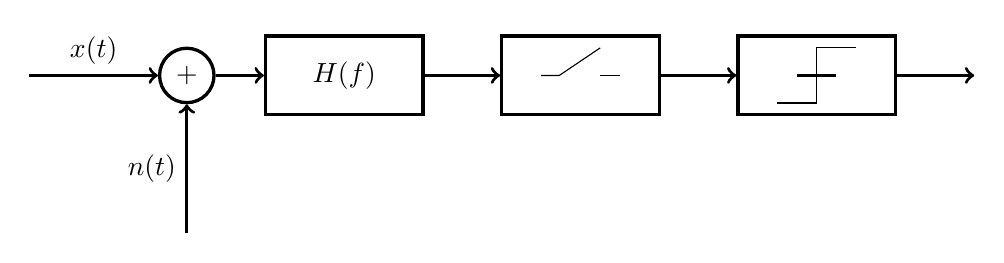
\begin{tikzpicture}[scale=2]
    \node[block](h)at(0,0){$H(f)$};
    \node[sum](+)at(-1,0){+};
    \draw[very thick,->](-2,0)--(+.180)node[midway, above]{$x(t)$};
    \draw[very thick,->](-1,-1)--(+.270)node[midway, left]{$n(t)$};
    \draw[very thick,->](+.0)--(h.180);
    \node[block](adc)at(1.5,0){};
    \node[block](s)at(3,0){};
    \draw[very thick,->](h.0)--(adc.180);
    \draw[very thick,->](adc.0)--(s.180);
    \draw[very thick,->](s.0)--(4,0);
    \draw(1.25,0)--(1.365,0)--(1.625,0.175);
    \draw(1.625,0)--(1.75,0);
    \draw(2.75,-0.175)--(3,-0.175)--(3,0.175)--(3.25,0.175);
    \draw[very thick](2.875,0)--(3.125,0);
\end{tikzpicture}
\end{document}